\documentclass[11pt,a4paper,twoside,onecolumn,titlepage]{report}
\usepackage[utf8]{inputenc}
\usepackage{ucs}
\usepackage{amsmath}
\usepackage{amsfonts}
\usepackage{amssymb}
\usepackage{enumerate}
\usepackage{listingsutf8}
\usepackage[numbered,autolinebreaks]{mcode}
\usepackage{caption}
\usepackage{pgfplotstable}
\usepackage{booktabs}
\usepackage{graphicx}
\usepackage{caption}
\usepackage{subcaption}
\usepackage[top=2cm, bottom=2cm, left=2cm, right=2cm]{geometry}

\graphicspath{{graphs/}}

\DeclareCaptionFont{white}{\color{white}}
\DeclareCaptionFormat{listing}{\colorbox{gray}{\parbox{\textwidth}{#1#2#3}}}
\captionsetup[lstlisting]{format=listing,labelfont=white,textfont=white}

\renewcommand{\thesection}{\arabic{section}}

\newcommand{\qn}{quasi-Newton}
\newcommand{\pfp}{plus forte pente}
\newcommand{\txtoptim}{\text{optim}}
\newcommand{\txtpfp}{\text{pfp}}
\newcommand{\txtcauchy}{\text{cauchy}}
\newcommand{\txtrchlin}{\text{rch lin}}
\newcommand{\txtqn}{\text{qN}}

\title{Résolution d'un problème d'optimisation différentiable}
\author{Marc \textsc{Bourqui} \and Victor \textsc{Constantin} \and Ian \textsc{Schori} \and Floriant \textsc{Simond}}

\lstset{
language=matlab,
extendedchars=\true,
inputencoding=utf8/latin1
}

% Le rapport a rendre pour le 11 janvier 2013 doit contenir:
% - Code Matlab
% - Expliquer les questions spécifiques du problème
% - Expliquer les comparaisons du problème
% - Les résultats







% TODO
%
% - mettre à jour les références, titres, labels, caption, etc.
% - logo EPFL première page
%
%






\begin{document}

%\maketitle
\newcommand{\HRule}{\rule{\linewidth}{0.5mm}}

\begin{titlepage}

\begin{center}


% Upper part of the page

\includegraphics[width=0.15\textwidth]{./images/epfl}\\[1cm]    

\textsc{\LARGE École Polytechnique Fédérale de Lausanne}\\[1.5cm]

\textsc{\Large Introduction à l'optimisation différentialbe}\\[0.5cm]


% Title
\HRule \\[0.4cm]
{ \huge \bfseries Résolution d'un problème}\\[0.4cm]

\HRule \\[1.5cm]


\begin{center}
Groupe 24\\
\ \\
Marc \textsc{Bourqui} \\ Victor \textsc{Constantin} \\ Ian \textsc{Schori} \\ Floriant \textsc{Simond}
\end{center}
% Author and supervisor
%\begin{minipage}{0.4\textwidth}
%\begin{flushleft} \large
%\emph{Author:}\\
%John \textsc{Smith}
%\end{flushleft}
%\end{minipage}
%\begin{minipage}{0.4\textwidth}
%\begin{flushright} \large
%\emph{Supervisor:} \\
%Dr.~Mark \textsc{Brown}
%\end{flushright}
%\end{minipage}

\vfill

% Bottom of the page
{\large \today}

\end{center}

\end{titlepage}

\section*{Énoncé du problème}

Trouver (une approximation de) la solution du problème suivant en appliquant le théorème de la plus forte pente:
\begin{equation}
\min_{x\in\mathbb{R}^2} (x_1-2)^4 + (x_1-2)^2x_2^2 + (x_2+1)^2
\end{equation}

\section*{Réponses aux questions}

\begin{enumerate}[(a)]
\item\label{pfp} Implémenter la méthode de plus forte pente (Algorithme 11.3) à l'aide du logiciel MATLAB. Déterminer la taille du pas en appliquant la recherche linéaire, Algorithme 11.2 (les deux conditions de Wolfe).

%
% Mettre la réponse ici
%
\lstinputlisting[label=pfp.m, caption=pfp.m]{pfp.m}
Pour \texttt{pfp.m}, nous avons réutilisé la structure du corrigé de la série 3. Nous l'avons adapté pour y résoudre la màthode de la plus forte pente, selon l'algorithme 11.3. La fonction, son gradient et sa hessienne sont placés dans un fichier que nous avons nommé \texttt{f.m}. De plus, nous avons ajouté un booléan \mcode{useRL} qui permet de sélectionner la méthode de détermination du pas (\mcode{true}~: recherche linéaire, \mcode{false}~: le pas calculé en (\ref{pas})).


\lstinputlisting[label=pfpInnerLoop.m, caption=pfpInnerLoop.m]{pfpInnerLoop.m}
Cette foction effectue une itération de l'algorithme de la \pfp\ en utilisant la méthode de calcul du pas spécifiée. Le choix est effectué à l'aide du booléen \mcode{useRL} qui permet de choisir entre la recherche linéaire et la méthode indiquée au point (\ref{pas}). Le paramètre \mcode{x0} est l'itéré précedent.

%
%TODO : Expliquer en qq mots ce que la recherche linéaire fait.
%
\lstinputlisting[label=rechercheLineaire.m, caption=rechercheLineaire.m]{rechercheLineaire.m}
Cette fonction implémente la recherche linéaire d'après l'algorithme 11.2. Le paramètre \mcode{fx} est la fonction évaluée en \mcode{x}, et le paramètre \mcode{gfx} est son gradient en \mcode{x}. Nous avons choisi de les passer en paramètres pour ne pas devoir les recalculer. Mais pour plus de modularité, on peut déterminer \mcode{fx} et \mcode{gfx} en ajoutant \mcode{[fx, gfx] = feval(f, x);} avant la boucle \mcode{while}.

%
%
%

\item\label{pas} Implémenter une fonction qui donne la taille du pas suivant:
\begin{equation}\label{eq:cauchy}
\alpha_k = \frac{\bigtriangledown f(x_k)^T \bigtriangledown f(x_k)}{\bigtriangledown f(x_k)^T \bigtriangledown^2 f(x_k) \bigtriangledown f(x_k)}
\end{equation}

Quelle est la nature de ce pas? D'où cette formule vient-elle?

%
% Mettre la réponse ici
%

\lstinputlisting[label=taillepasCauchy.m, caption=taillepasCauchy.m]{taillepasCauchy.m}

   
%Cette formule est le point de Cauchy. Elle vient du modèle quadratique. C'est le point qui minimise le modèle quadratique de la fonction dans la direction de la plus forte descente.
Comme $f$ n'est pas une fonction linéaire, on peut l'approximer par un modèle quadratique.
On va chercher à miniser ce modèle dans la direction de la plus forte descente, à savoir $\bigtriangledown f$. Le point qui minimise ce modèle est le point de Cauchy et se détermine de la manière suivante~:
\begin{equation}
x_C = x_k - \alpha_C \bigtriangledown f(x_k)
\end{equation}
où
\begin{equation}
\alpha_C = \underset{\alpha \in \mathbb{R}^+_0}{\operatorname{argmin}}\ m_{x_k}(x_k-\alpha\bigtriangledown f(x_k))
\end{equation}
Sachant $f$ convexe, $\alpha_C$ peut être calculé par \eqref{eq:cauchy}.




%
%
%

\item\label{questionC} Comparer le comportement de l'algorithme en utilisant les pas (\ref{pfp})\ et (\ref{pas}).

%
% Mettre la réponse ici
%
Pour comparer ces deux méthodes, nous avons choisi d'utiliser comme critère le nombre d'itérations que prend chacun. 

Pour pouvoir repondre aux questions \ref{questionC}\ et \ref{questionD}\ nous avons créé un fichier MatLab, \texttt{comparator.m}, qui nous permet de lancer deux méthodes l'une après l'autre et qui enregistre les résultats. Il génère aussi un tableau contenant le nombre d'itérations pour chaque méthode et des graph, ceci dans le but de nous faciliter la comparaison.

Afin de comparer les pas, il faut mettre \mcode{compareSteps = true} dans \texttt{compartor.m}. Pour générer le tableau \ref{t1} , nous avons défini arbitrairement 10 vecteurs \mcode{x} dans le fichier \texttt{x.m}.

\begin{figure}
\pgfplotstabletypeset[
col sep=comma,
string type,
columns/0/.style={column name=},
columns/1/.style={column name=},
columns/2/.style={column name=},
columns/3/.style={column name=},
columns/4/.style={column name=},
columns/5/.style={column name=},
columns/6/.style={column name=},
columns/7/.style={column name=},
columns/8/.style={column name=},
columns/9/.style={column name=},
columns/10/.style={column name=},
every head row/.style={before row={\toprule $k$ & \multicolumn{2}{c}{$x_0$} & \multicolumn{2}{c}{$x_{\txtoptim,\txtrchlin}$} & $f(x_{\txtoptim,\txtrchlin})$ & $n_{\txtrchlin}$ & \multicolumn{2}{c}{$x_{\txtoptim,\txtcauchy}$} & $f(x_{\txtoptim,\txtcauchy})$ & $n_{\txtcauchy}$ \\
}
},
every last row/.style={after row=\hline},
]{compareSteps.csv}
\caption{Recherche linéaire vs. pas de Cauchy}\label{t1}
\end{figure}

Afin d'avoir plus de valeurs nous avons défini une fonction en colimaçon dans le fichier \texttt{xsnake.m}, qui génère une suite de points commencant à la solution ( $(2,-1);\ (3,-1);\ (3,0);\ (-1,0);\ (1,-2);\ \ldots$ ). Nous l'avons utilisé pour générer beaucoup de points afin d'avoir des valeurs pour nos graph.

Dans la figure \ref{rlVSqn}\ nous avons un premier graph avec 500 valeurs.

\begin{figure}[h!]
	\centering
	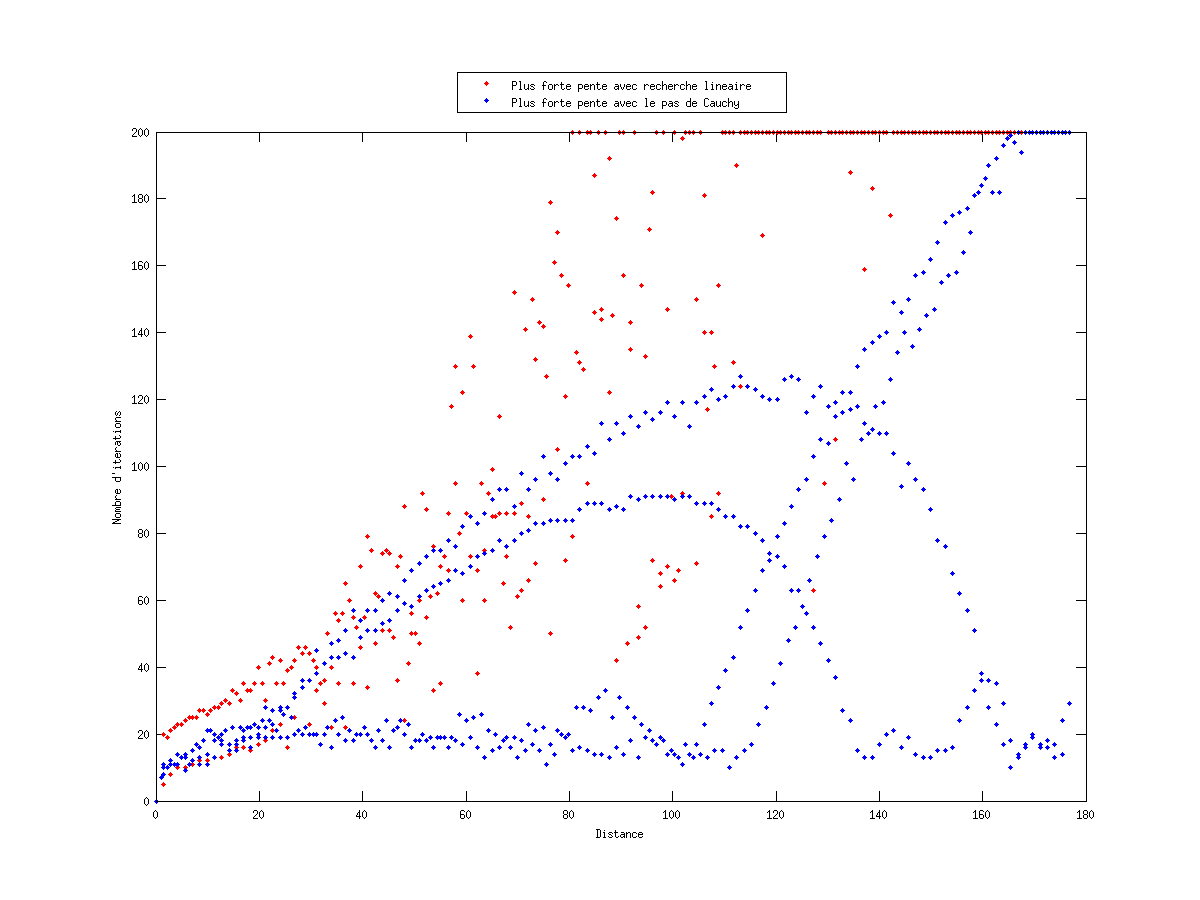
\includegraphics[scale=0.9]{steps-allinone}
	\caption{Recherche linéaire vs. quasi-Newton}
	\label{rlVSqn}
\end{figure}


%\noindent\makebox[0.9\textwidth]{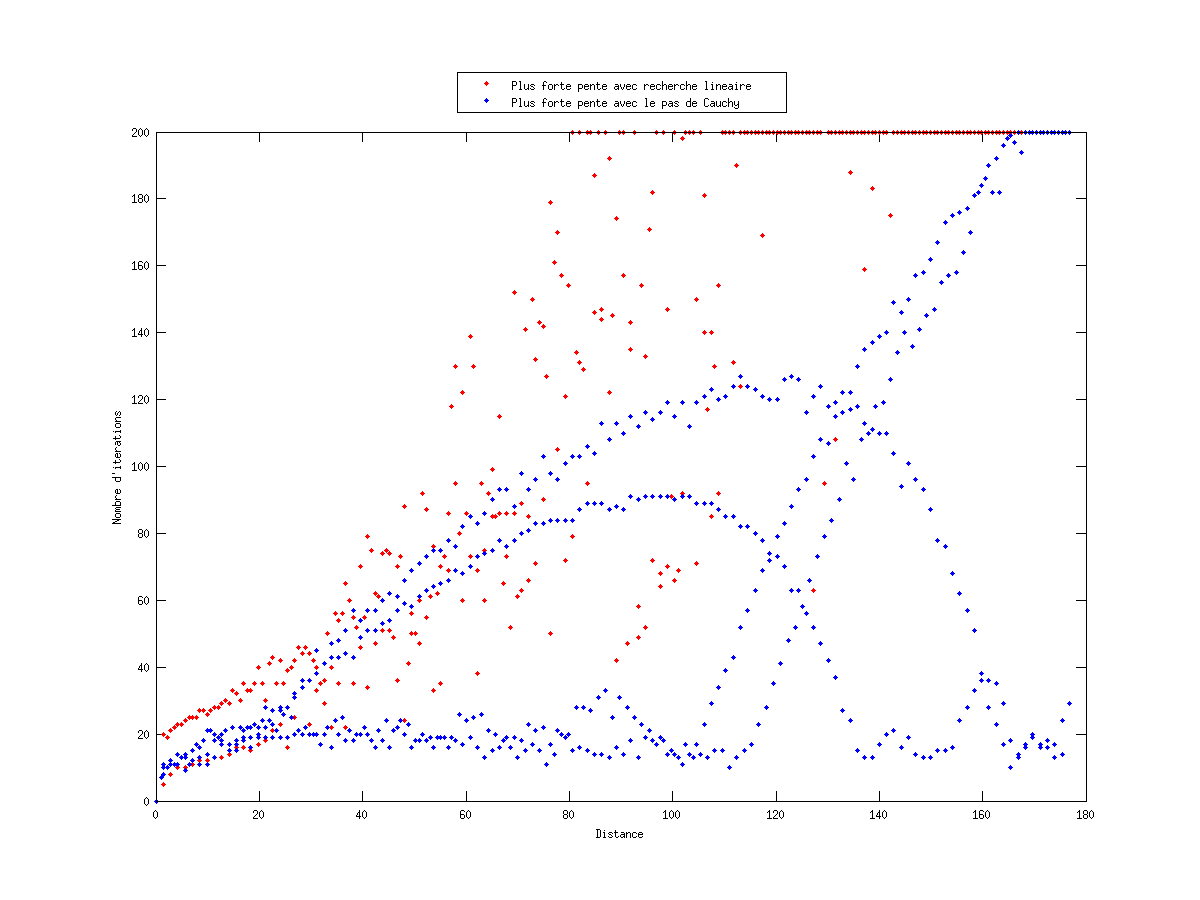
\includegraphics[width=1.3\textwidth]{steps-allinone}\label{fig:awesome_image}}


Ce graphique n'est pas très explicite, mais on observe tout de même la tendance générale de la méthode de plus forte pente avec la recherche linéaire qui nécessite beaucoup d'itérations lorsque la distance à la solution est grande. L'utilisation du pas de Cauchy permet d'améliorer grandement l'efficaticité de l'algorithme, en particulier pour de grandes distances. Toutefois, on remarque deux tendances, dont l'une tend à être inefficace tandis que l'autre reste efficace.



Nous avons séparé les résultats selon les différences de coordonnées du point de départ par rapport à la solution. Nous avons représenté les valeurs sur la figure \ref{fig:steps-4}.

\begin{figure}[h!]
    \centering
	\begin{subfigure}[t]{0.5\textwidth}
		\centering
		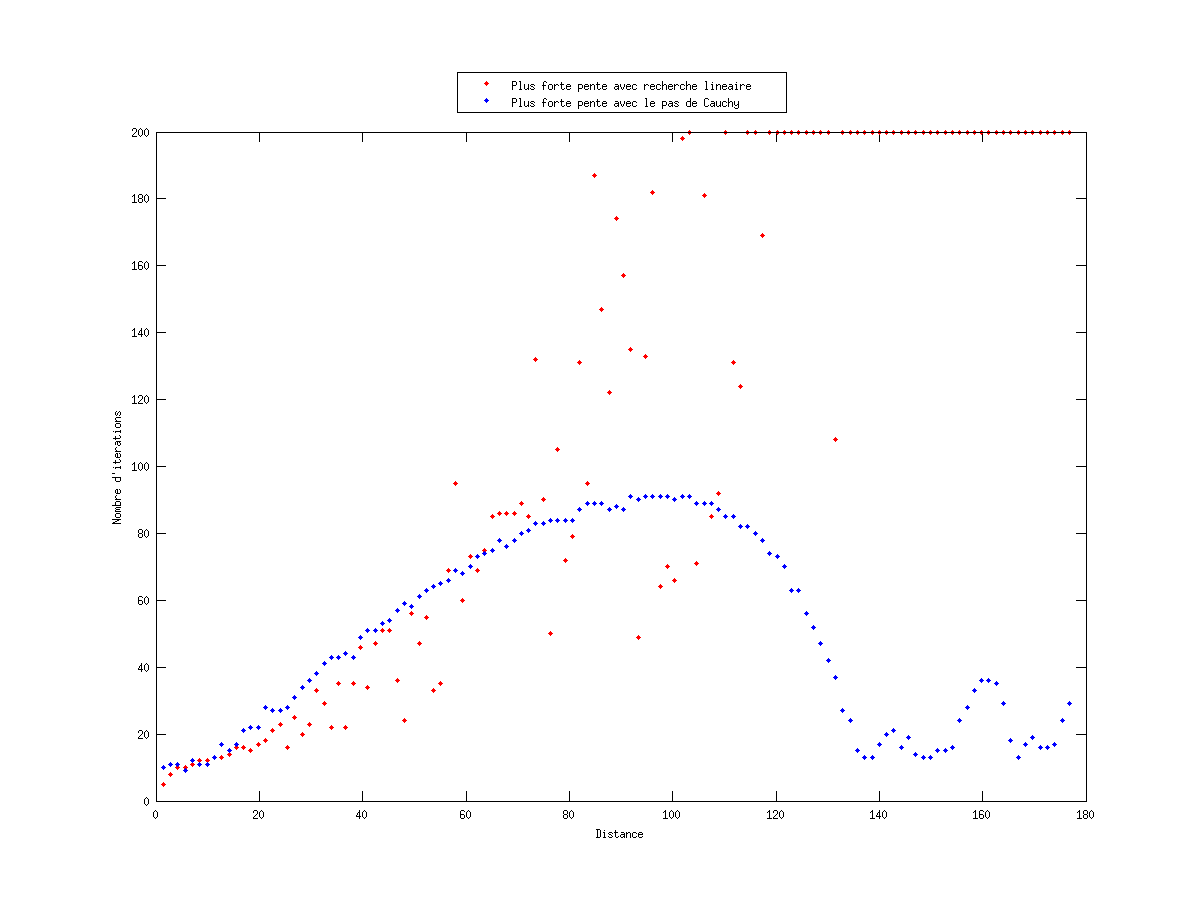
\includegraphics[scale=0.4]{steps-quarter-4}
		\caption{-x +y}
		\label{fig:rlVSqnQ4}
	\end{subfigure}%
        ~ %add desired spacing between images, e. g. ~, \quad, \qquad etc. 
          %(or a blank line to force the subfigure onto a new line)
    \begin{subfigure}[t]{0.5\textwidth}
		\centering
		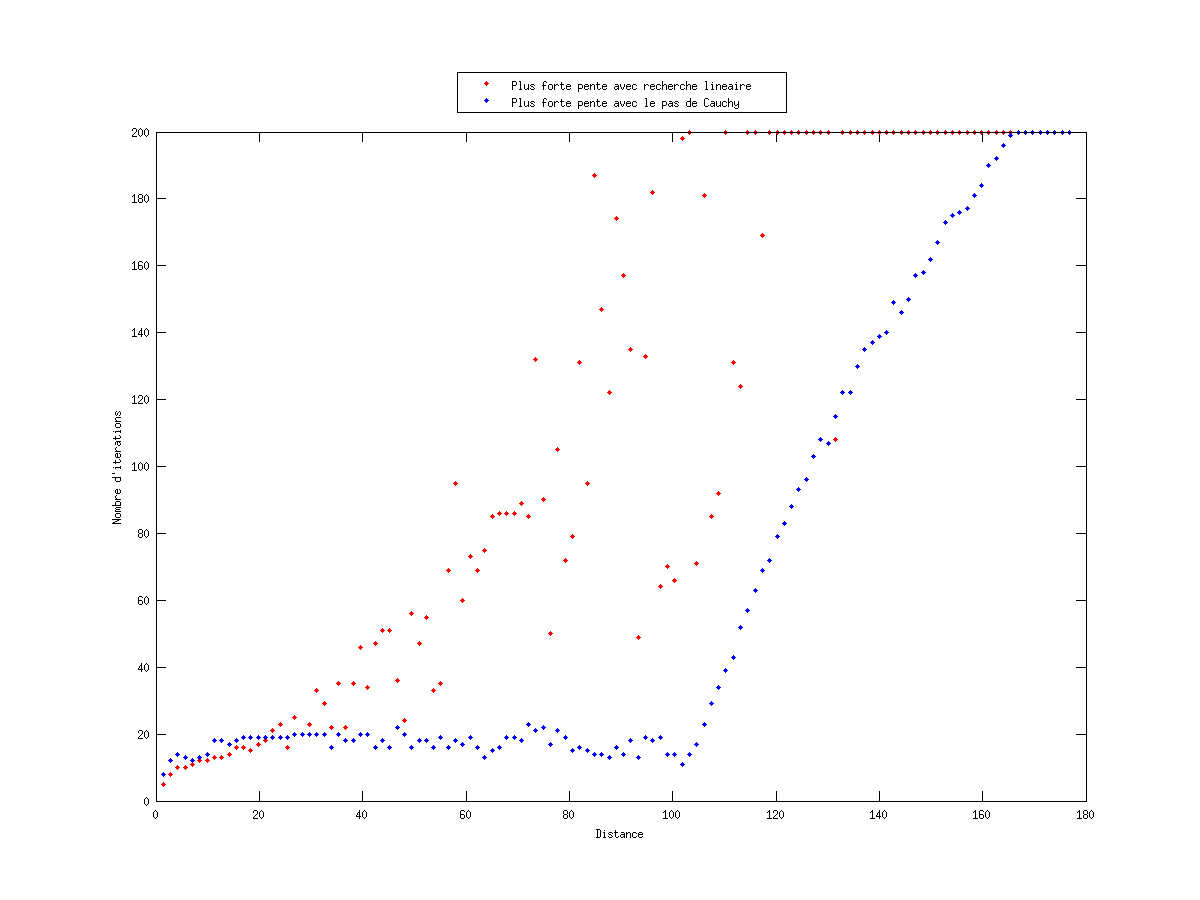
\includegraphics[scale=0.4]{steps-quarter-3}
		\caption{+x +y}
		\label{fig:fig:rlVSqnQ3}
	\end{subfigure}

	\begin{subfigure}[t]{0.5\textwidth}
		\centering
		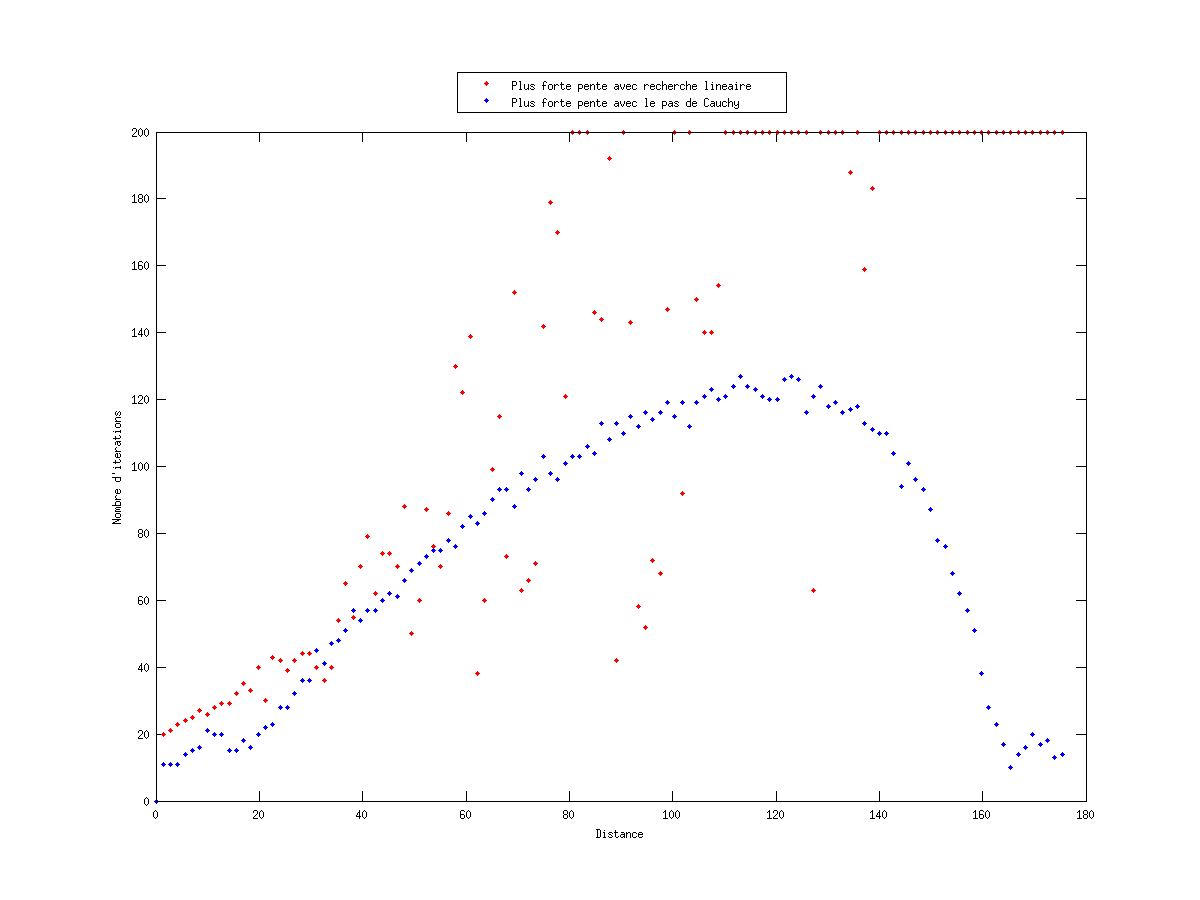
\includegraphics[scale=0.4]{steps-quarter-1}
		\caption{-x -y}
		\label{fig:fig:rlVSqnQ1}
	\end{subfigure}%
        ~ %add desired spacing between images, e. g. ~, \quad, \qquad etc. 
          %(or a blank line to force the subfigure onto a new line)
    \begin{subfigure}[t]{0.5\textwidth}
		\centering
		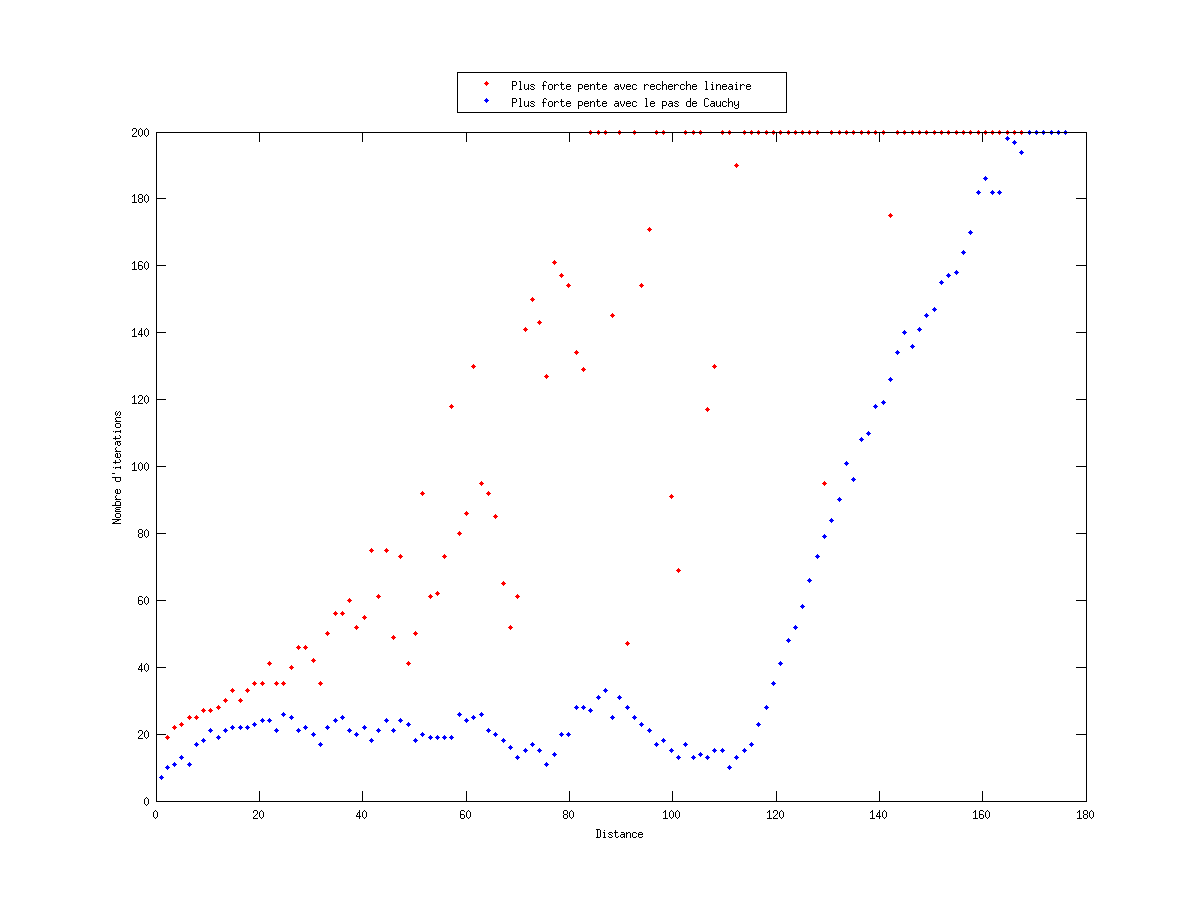
\includegraphics[scale=0.4]{steps-quarter-2}
		\caption{+x -y}
		\label{fig:fig:rlVSqnQ2}
	\end{subfigure}
    \caption{Graphs comparaison recherche linéaire vs. Cauchy par quadrant}\label{fig:steps-4}
\end{figure}


On remarque que lorsque x est diminuée, l'alogrithme utilisant le pas de Cauchy est bien plus efficace que la recherche linéaire, en particulier pour de grandes distances à la solution. Alors que lorsque x est augmenté, cette méthode reste généralement meilleure que la recherche linéaire. Cependant, son efficacité est grandement réduite pour de grandes distances.

On notera aussi que l'algorithme utilisant le pas de Cauchy change de comportement selon le décalage sur x. En effet, jusqu'à la centaine, lorsque que x est dédéuit, l'algorithme perd en efficacité, alors que lorsque x est ajouté, l'algorithme est stable. Mais à partir d'une distance supérieure à la centaine, l'inverse se produit.

%
%
%


\item\label{questionD} Comparer la methode de plus forte pente et la methode quasi-Newton (qui est déjà implementée -- Série 3).

%
% Mettre la réponse ici
%

\begin{figure}
\pgfplotstabletypeset[
col sep=comma,
string type,
columns/0/.style={column name=},
columns/1/.style={column name=},
columns/2/.style={column name=},
columns/3/.style={column name=},
columns/4/.style={column name=},
columns/5/.style={column name=},
columns/6/.style={column name=},
columns/7/.style={column name=},
columns/8/.style={column name=},
columns/9/.style={column name=},
columns/10/.style={column name=},
every head row/.style={before row={\toprule $k$ & \multicolumn{2}{c}{$x_0$} & \multicolumn{2}{c}{$x_{\txtoptim,\txtpfp}$} & $f(x_{\txtoptim,\txtpfp})$ & $n_{\txtpfp}$ & \multicolumn{2}{c}{$x_{\txtoptim,\txtqn}$} & $f(x_{\txtoptim,\txtqn})$ & $n_{\txtqn}$ \\
}
},
every last row/.style={after row=\hline},
%every first column/.style={column type/.add={>{\makebox[3em][l]{\arabic{myCounter}\stepcounter{myCounter}~}}}{} }
]{compareMethods.csv}
\caption{Plus forte pente vs. Quasi-Newton}\label{t2}
\end{figure}


D'une manière générale, la méthode de la plus forte pente est plus efficace que la méthode de quasi-Newton lorsque la distance entre le point de départ et la solution est petite.


Pour se faire une idée du comportement des deux méthodes, nous avons générés 350 valeurs de départ d'après notre méthode \mcode{xsnake}. Le résultat est présenté sur la figure \ref{fig:pfp-vs-qn}.


\begin{figure}[h!]
	\centering
	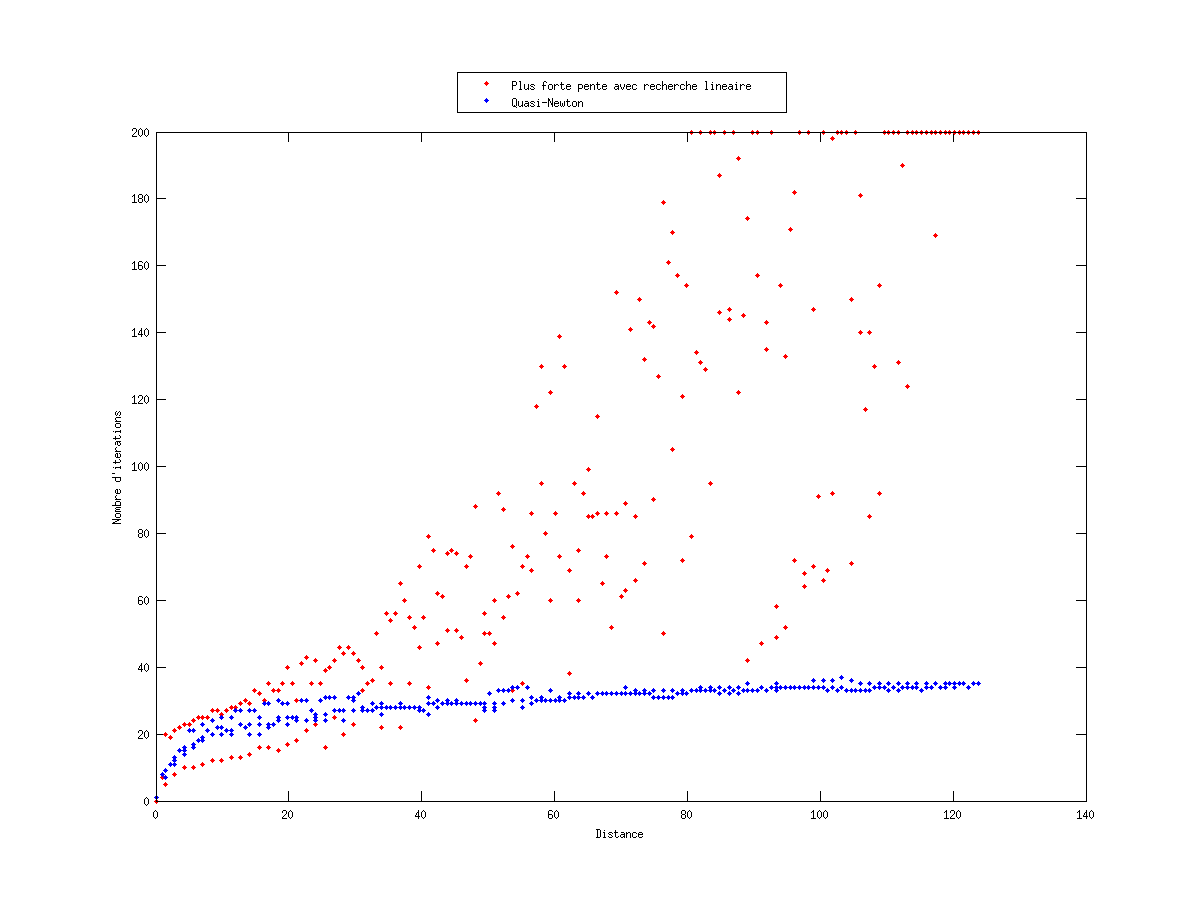
\includegraphics[scale=0.9]{methods-allinone}
	\caption{PFP VS Quasi-Newton}
	\label{fig:pfp-vs-qn}
\end{figure}

Au premier coup d'oeil, on observe que la méthode quasi-Newton est plus efficace que la méthode de plus forte pente. Toutefois, la méthode de plus forte pente est en moyenne une fois sur deux plus efficace à proximité de la solution.

Pour distinguer plus clairement ces différences, nous avons séparé les résultats selon les 4 mêmes cadrans qu'au point \ref{questionC}.




\begin{figure}[h!]
    \centering
	\begin{subfigure}[t]{0.5\textwidth}
		\centering
		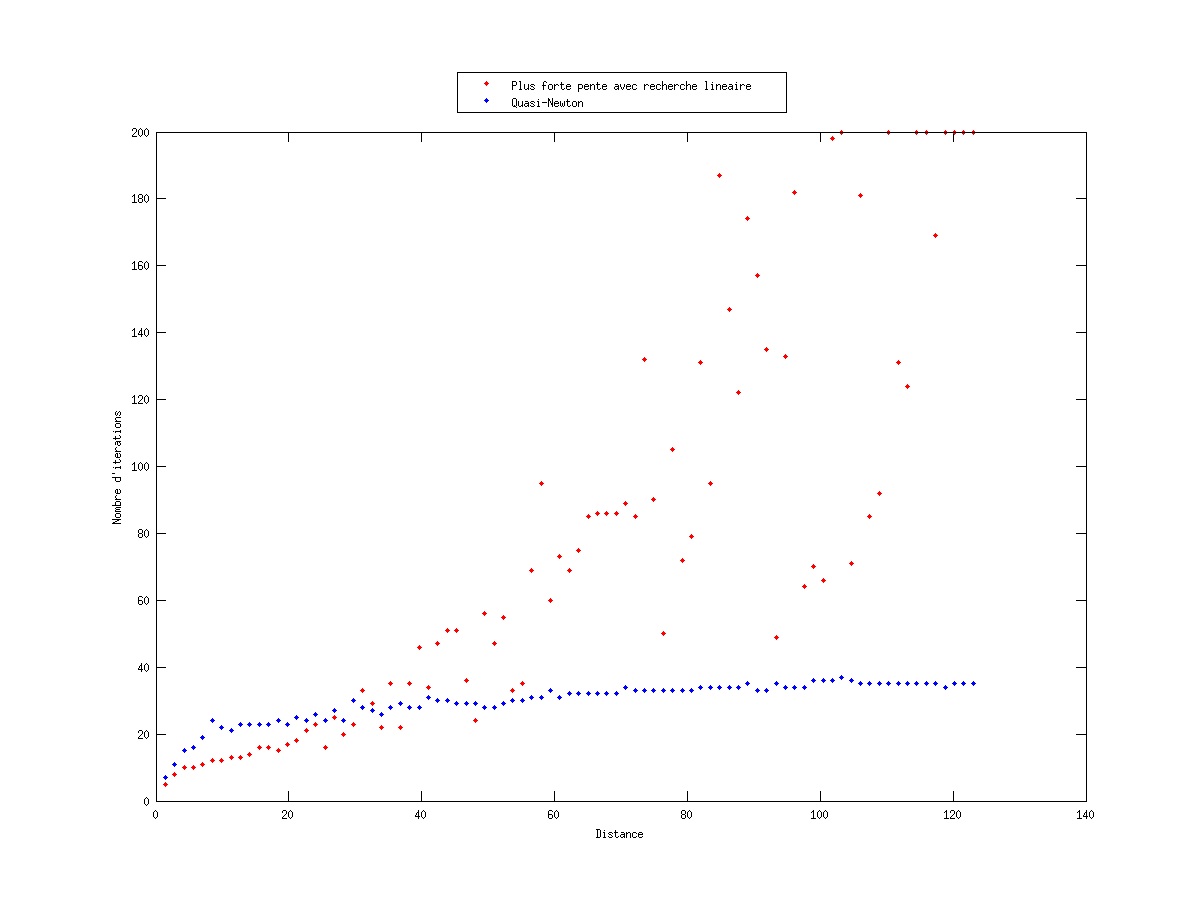
\includegraphics[scale=0.4]{methods-quarter-4}
		\caption{-x +y}
		\label{fig:awesome_image}
	\end{subfigure}%
        ~ %add desired spacing between images, e. g. ~, \quad, \qquad etc. 
          %(or a blank line to force the subfigure onto a new line)
    \begin{subfigure}[t]{0.5\textwidth}
		\centering
		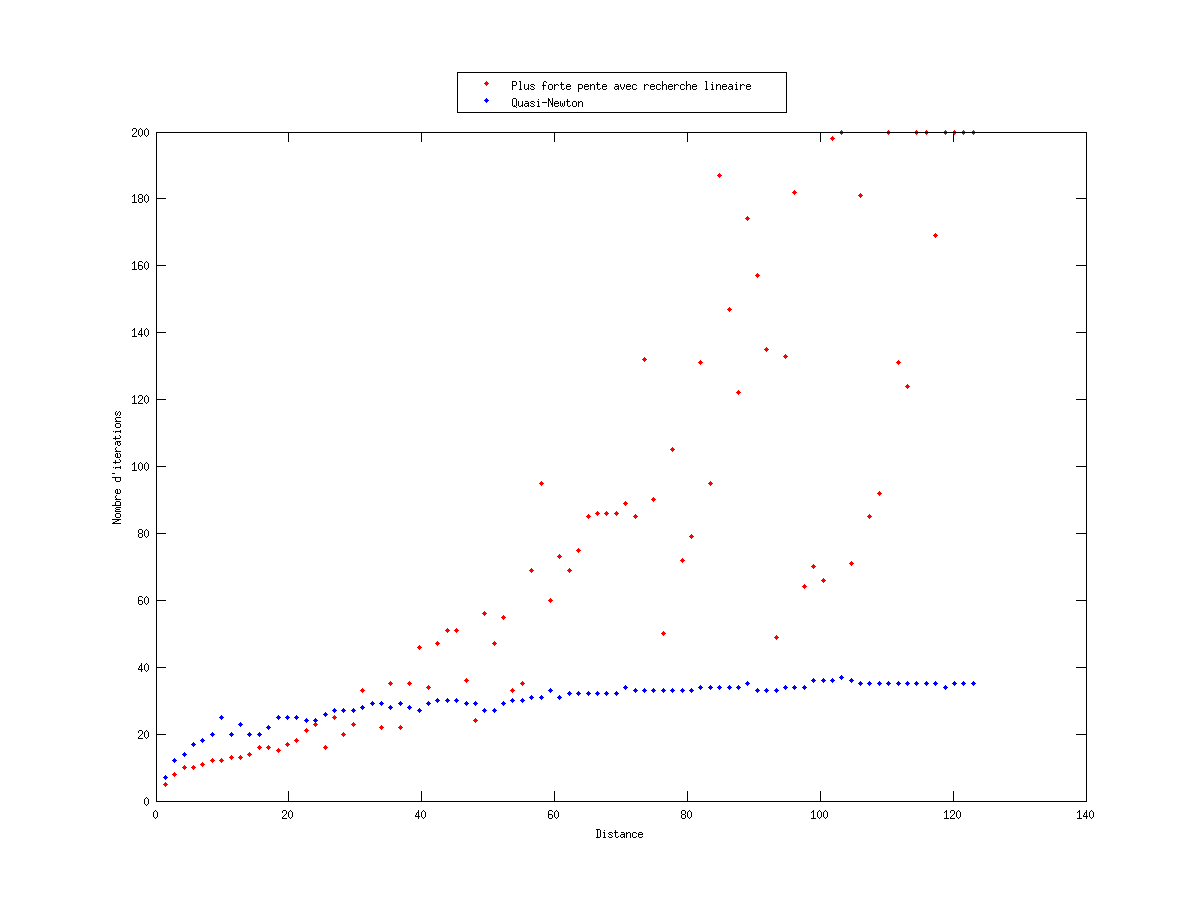
\includegraphics[scale=0.4]{methods-quarter-3}
		\caption{+x +y}
		\label{fig:awesome_image}
	\end{subfigure}

	\begin{subfigure}[t]{0.5\textwidth}
		\centering
		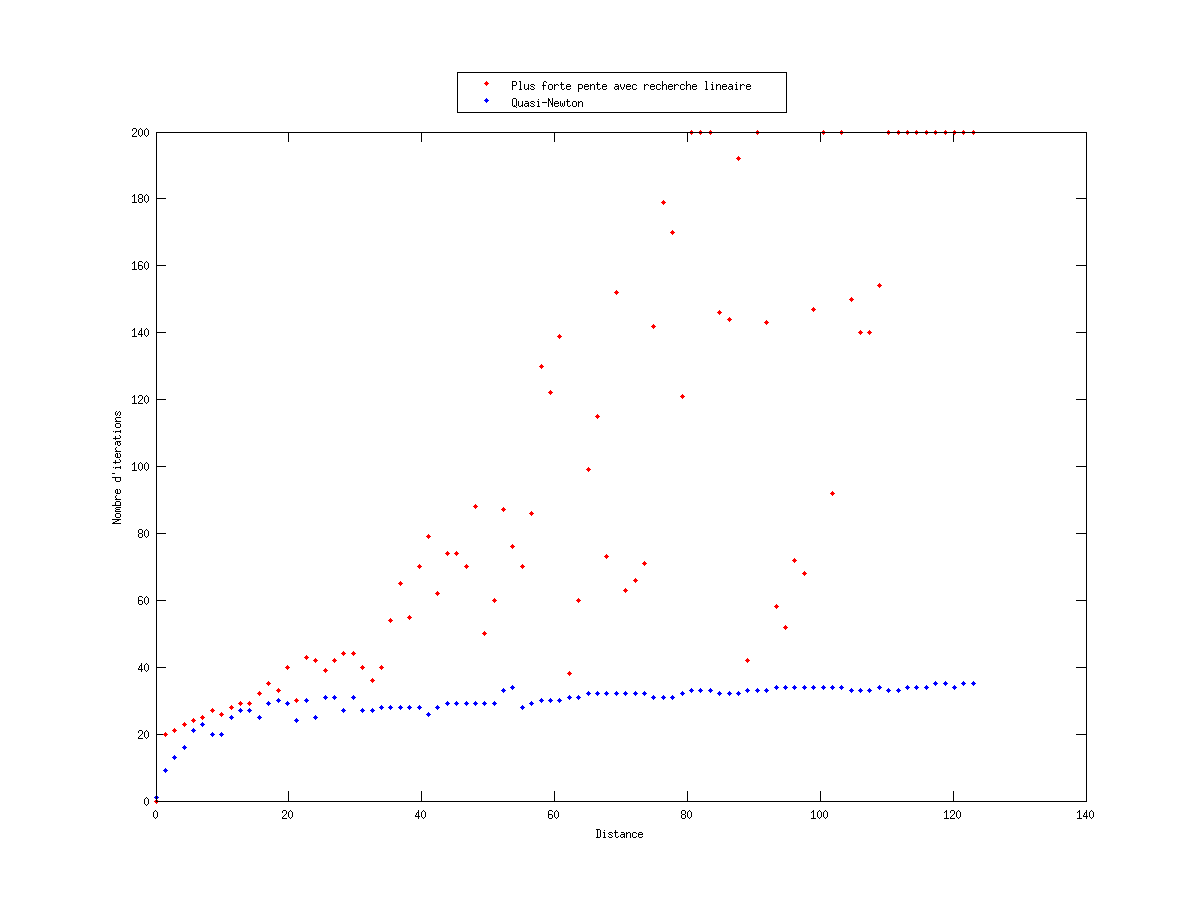
\includegraphics[scale=0.4]{methods-quarter-1}
		\caption{-x -y}
		\label{fig:awesome_image}
	\end{subfigure}%
        ~ %add desired spacing between images, e. g. ~, \quad, \qquad etc. 
          %(or a blank line to force the subfigure onto a new line)
    \begin{subfigure}[t]{0.5\textwidth}
		\centering
		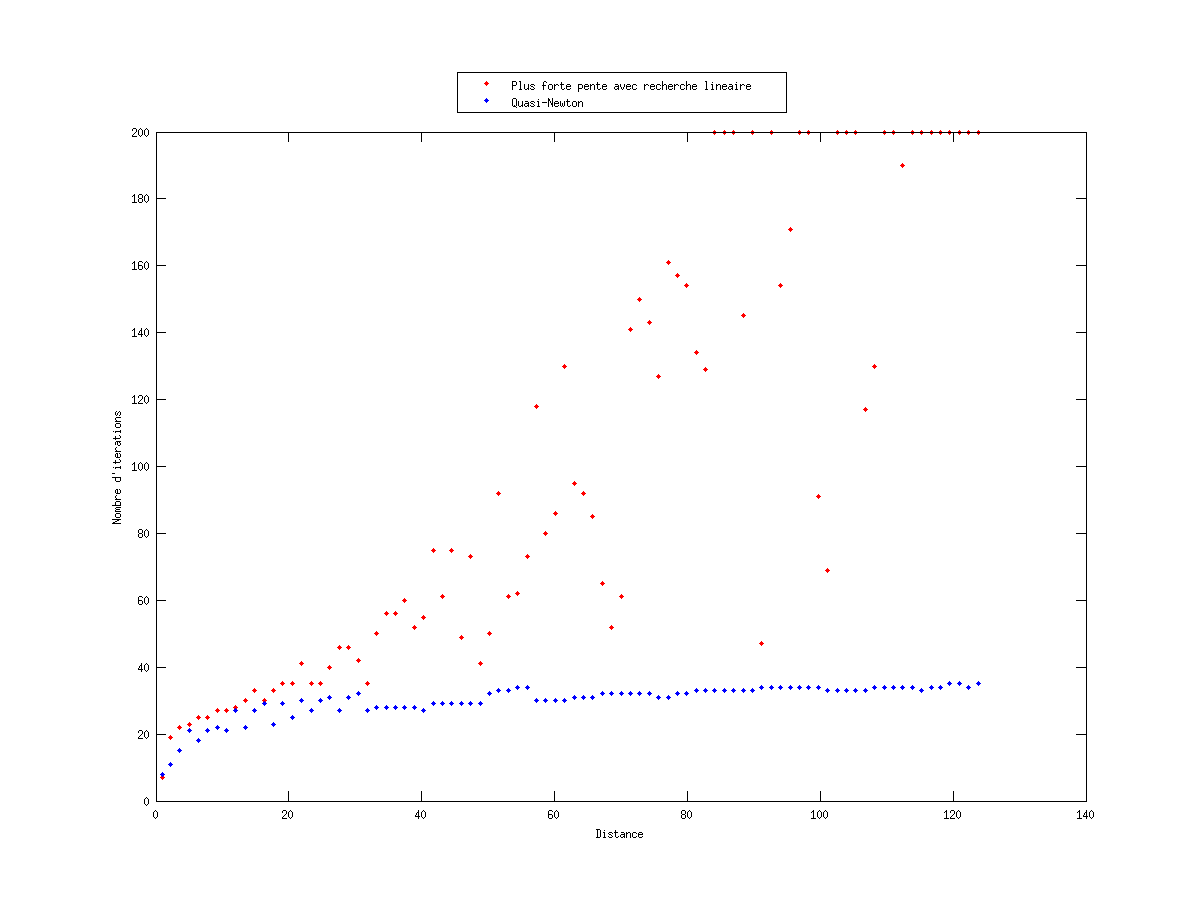
\includegraphics[scale=0.4]{methods-quarter-2}
		\caption{+x -y}
		\label{fig:awesome_image}
	\end{subfigure}
    \caption{Graphs comparaison plus forte pente vs. Quasi-Newton par quadrant}\label{fig:methods-4}
\end{figure}


On remarque que lorsque l'on s'éloigne de la solution en augmentant y, la méthode de \pfp\ est plus appropriée à proximité de la solution. Mais à partir d'une distance à la solution de 40 environ, la méthode de \qn\ devient plus performante.

Par contre, lorsque l'on s'éloigne selon $-y$, la méthode de \pfp\ est quasiment constamment plus inefficace.

La méthode de \qn\ semble se stabiliser assez rapidement et le nombre d'itérations augmente très légérement. Alors que la méthode de \pfp\ donne des résultats aléatoires.


\end{enumerate}
\end{document}